\section{Module 10. Upsampling}

The implementation began with making a decision about the input data. The input image has to be 2 dimensional without a noise. The uploaded image will be considered as a 2 dimensional array of double values. Other parameters that will be needed are vertical and horizontal extensions. It has to be a total number. The size of the input array will be multiplied by the number. For example, the image 256x256 pixels with extensions equal to 3 will be 768x768 pixels as an output. The function needs also the window size. In one iteration, the function will take into consideration only pixels witch are inside the window. The loop will stop only when the whole image will be interpolated. To see the results the \textit{plotting} parameter has to be a boolean \textit{True} value. 
\newline The below picture shows the block diagram of the algorithm (Fig. \ref{fig: Module10_4}) with comments added.

\begin{figure}[H]
\centering{}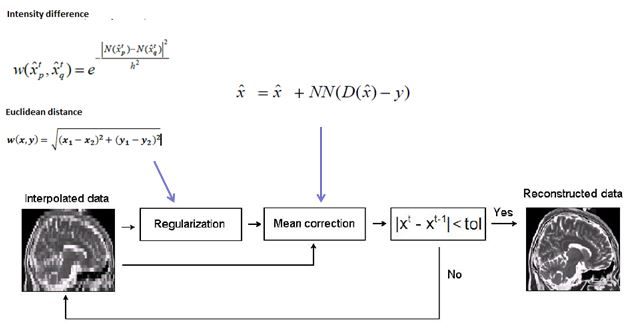
\includegraphics[scale=0.7]{figures/Module_10/Module10_4}\caption{Algorithm block diagram with comments}. 
\label{fig: Module10_4}
\end{figure}

The following steps of the implementation will be discussed:

\begin{enumerate}

\item \textbf{Initial interpolation}
\newline To form the input image into the output with chosen size the initial interpolation is needed. As showed in \cite{9art1} the spline interpolation is used. In short, spline interpolation is an interpolation where interpolant is a special kind of piecewise polynomial called spline. It is recommended, because of the fact that the method makes small error even with low degree polynomials for the spline. Taking into consideration the edges the extrapolation was applied. To be more specific, the last row \textit{n} is equal to the previous one \textit{n-1}. The same with the first row, the first column and the last column of the input. To show the results, the extensions are set as 2. The input data is 256x256 pixels. The undermentioned picture (Fig. \ref{fig: Module10_5}) shows the result of the initial interpolation. The scale is included so it is easy to see that the size is twice as big. Now, the zeros (Fig. \ref{fig: Module9_3}) have  nonzero values, so the next steps can be made.


\begin{figure}[H]
\centering{}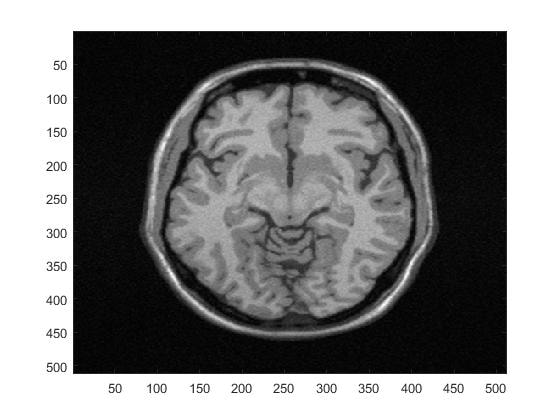
\includegraphics[scale=0.5]{figures/Module_10/Module10_5}\caption{The image after initial interpolation 512x512 pixels}. 
\label{fig: Module10_5}
\end{figure}

\item \textbf{Regularization}
\newline The main functionality is the regularization step. The function makes the square window which contains some pixels. In one iteration of a loop, only the pixels which are inside the window are considered. Next, the window moves and takes another pixels. It is repeated till the end of the image. The main goal is to determine of the weight which will be used at the end.
\newline The first weight is calculated as the difference between the pixels intensities.
\newline 
\centerline {$w_{1}(x, y)= e^{\frac{|N(x)-N(y)|^{2}}{h^{2}}}$, where}
\newline
\newline $N(x)$, $N(y)$ are window and image intensity values,
\newline $h$ is a level, which is equal to the half of the standard deviation of the input image.
\newline The next part of the whole weight is an Euclidean distance weight. It is simply calculated as the Euclidean distance between every pixel in the window and every pixel in the image. It is based on the below equation.
\newline
\centerline{ $w_{2}(x,y)=\frac{\sqrt{(x_{1}-x_{2})^{2}+(y_{1}-y_{2})^{2}}}{h^{2}}$, where }
\newline
\newline $h$ is a level, which is equal to the half of the standard deviation of the input image.
\newline The total weight is calculated as $w_{total}=w_{1}*w_{2}$. The output image is determined as the result of the sum of the multiplication of the weight and the window, divided by the sum of the weight.

\item \textbf{Mean correction}
\newline The mean correction step is a place in the function where the correctness of the equation $X=X+NN*(D(X)-y)$. It was abovementioned, that the downsampled HR has to be equal to the input data.

\item \textbf{Tolerance checking}
At the beginning it was established that only the 2D images will be taken into consideration and the upsampling function will be applied only once, so the step is excluded. There were experiments to upsample the data several times, but the result were not satisfied.

\end{enumerate}
